\chapter{Data}
\clearpage

\section{Types of Data}
	
	\begin{itemize}
		\item {\bf Data set: } collection of data objects.
		\item {\bf Data Objets: } often called record, point, vector, pattern, event, case,
		sample, observation or entity. Data objects are described by a number of attributes
		that capture the basic characteristics of an object.
		\item {\bf Attributes: } other names used are variable, characteristic, field, feature, 
		or dimension. An attribute is a property or characteristic of an object that may
		vary, either from one object to another or from time to another.
		\item {\bf Measurement scale: } is a rule (function) that associates a numerical or
		symbolic value with an attribute of an object. It is important to understand the 
		mesurement. An attribute can be an integer like ID and age. They are both integers, 
		but it does not mean that we can calculate the average ID numer like we can calculate
		the average age. Note that is common to refer to the type of an attribute as the
		{\bf type of a measurement scale}.
	\end{itemize}

	\subsection*{Types of Attributes}
	{\bf Categorical types (Qualitative):} Nominal and Ordinal

	{\bf Numeric types (Quantitative):} Interval and Ratio

		\begin{figure}[H]
			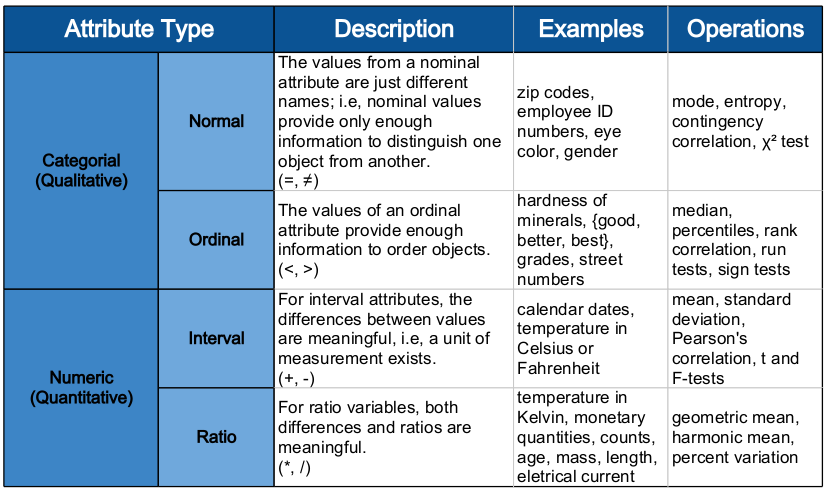
\includegraphics[width=\textwidth]{pics/typeOfAttributes.png}
		\end{figure}

	\clearpage
	\subsection*{Transformations}

		The types of attributes can be described in terms of transformations that
		do not change the meaning of an attribute. 

		\begin{figure}[H]
			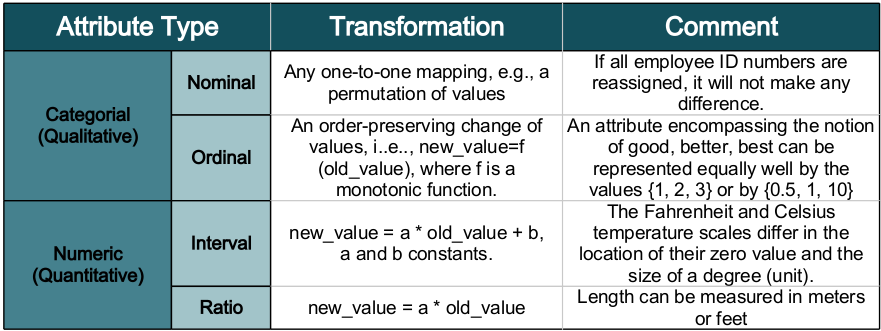
\includegraphics[width=\textwidth]{pics/transformations.png}
		\end{figure}

	\subsection*{Attributes by the Number of Values}

	An independent way of distinguishing between attributes is by the number of values
	they can take.

	\begin{itemize}
		\item {\bf Discrete:} A discrete attribute has a finite or countably infinite
		set of values. {\bf Binary attributes} are a special case of discrete attributes. 
		\item {\bf Continnuous:} A continuous attribute is one whose values are real numbers.
		\item {\bf Asymmetric:} For asymmetric attributes, only presence - a non-zero attribute
		value - is regarded as important. Binary attributes where only non-zero values are 
		important are called asymmetric binary attibutes. We can take a look at a list of all 
		courses at NTNU. If we look at a particular student, the chance for a particular student
		have taken a exam in a course from the whole list is quite small. It is only the non-zero
		values that are important. 
	\end{itemize}

	\clearpage
	\section{Type of Data Sets}

		\subsection*{General Characteristics of Data Sets}
			\begin{itemize}
				\item {\bf Dimensionality:} is the number of attributes that the object in the 
				class set possess.
				\item {\bf Sparsity:} for some data sets, such as asymmetric features, most
				attributes of an object have values of 0. In practical terms, sparsity is an advantage
				because usually only the non-zero values need to be stored an manipulated. 
				\item {\bf Resolution:} it is frequently possible to obtain data at different levels of
				resolution, and often the properties of the data are different at different resoultions.
				F.eks the surface of the Earth seems very uneven at a resolution of a few meters, but is *
				relatively smooth at a resolution of ten kilometers. The patterns in the data also depend
				on the level of resolution. Too fine will might hide the pattern or be buried in noise if
				to uneven. 
			\end{itemize}


		\clearpage
		\subsection*{Record Data}
		Much data mining work assumes that the data set is a collection of records (data objects), each of which consists of a fixed set of data fields (attributes).
			\begin{itemize}
				\item {\bf Transactions or Market Basket Data:} transaction data is a sepecial type of record
				data, where each record (transaction) involves a set of items. Transaction data is a collection
				of sets of items. 
				\item {\bf The Data Matrix:} if the data objects in a collection of data all have the
				same fixed set of numeric attributes, then the data objects can be thought of as points
				(vectors) in a multidimensional space, where each dimension represents a distinct attribute
				describing the object. 
				\item {\bf The Sparse Data Matrix:} A sparse data matrix is a special case of a data matrix in
				which the attributes are some of the same type and are symmetric; i.e, only non-zero values
				are important. {\bf Document-term matrix } is one type. 
			\end{itemize}

		\begin{figure}[H]
			\centering
			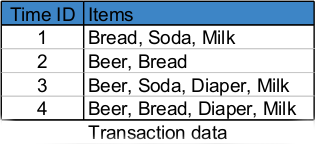
\includegraphics[scale=0.5]{pics/transactionData.png}
		\end{figure}

		\begin{figure}[H]
			\centering
			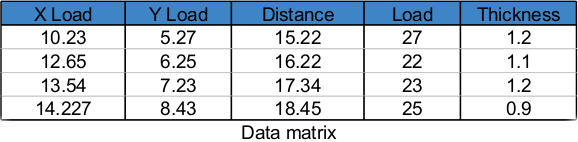
\includegraphics[scale=0.5]{pics/dataMatrix.png}
		\end{figure}

		\begin{figure}[H]
			\centering
			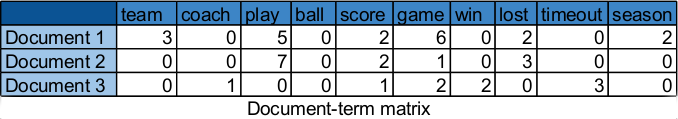
\includegraphics[scale=0.5]{pics/DocumentTermMatrix.png}
		\end{figure}

		\subsection*{Graph-Based Data}
			\begin{itemize}
				\item {\bf Data with Relationships among Objects:} the relationships among objects frequently convey important information. In such cases, the data is often represented as a graph. In 
				particular, the data objects are mapped to nodes of the graph, while the relationships among
				objects are captured by the links between objects and link propeties. 
				\item {\bf Data with Objects Thar Are Graphs:} if objects have structure, that is, the objects
				contain subobjects that have relationships, then such objects are frequently represented as graphs.
			\end{itemize}

		\clearpage
		\subsection*{Ordered Data}
		For some types of data, the attributes have relationships that involve order in time or space. 
			\begin{itemize}
				\item {\bf Sequential Data (temporal data):} can be thought of as an extension of record data, 
				where each record ha a time associated with it. 
				\item {\bf Sequence Data:} consists of a data set that is a sequence of individual entities, 
				such as a sequence of words or letters. 
				\item {\bf Time Series Data:} is a special type of sequential data in which each record is a
				time series, i.e, a series of measurements taken over time. 
				\item {\bf Spatial Data:} some objects have spatial attributes, such as positions or areas, as
				well as other type of attributes. 
			\end{itemize}

		\begin{figure}[H]
			\centering
			\subfigure{
				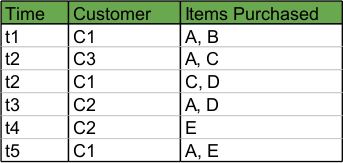
\includegraphics[scale=0.5]{pics/transactionData1.png}
			}
			\subfigure{
				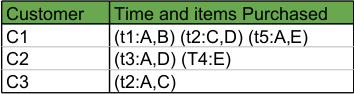
\includegraphics[scale=0.5]{pics/transactionData2.png}
			}
			\caption{Sequential transaction data}
		\end{figure}

		\begin{figure}[H]
			\centering
			\subfigure{
				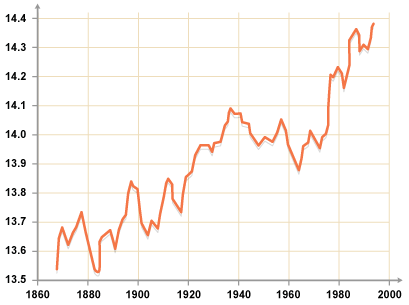
\includegraphics[scale=0.4]{pics/timeSeries.png}
			}
			\subfigure{
				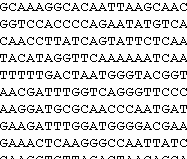
\includegraphics[scale=0.7]{pics/GenomicSequence.png}
			}
			\caption{Temperature time series and Genomic sequence data}
		\end{figure}

		\begin{figure}[H]
			\centering
			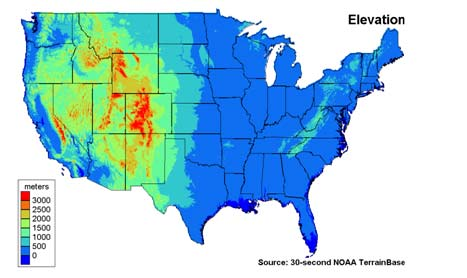
\includegraphics[scale=0.5]{pics/spatialTemp.jpg}
			\caption{Spatial temperature data}
		\end{figure}


\section{Data Quality}
	
	{\bf Data mining focuses on:}
	\begin{enumerate}
		\item The detection and correction of data quality problems (data cleaning).
		\item The use of algorithms that can tolarate poor data quality
	\end{enumerate}

	{\bf Measurement error:}
		\begin{itemize}
			\item {\bf Noise}
			\item {\bf Artifacts:} data errors may be the result of a more deterministic
			phenomenon, such as a streak in the same place on a set of photographs.
			\item {\bf Bias:} a systematic variation of measurements from the quanity
			being measured. 
			\item {\bf Precision:} the closeness of repeated measurements (of the
			same quantity) to one another.
			\item {\bf Accuracy:} the closeness of measurements to the true value
			of quantity being measured.
		\end{itemize}

	{\bf Data collection problems:}
		\begin{itemize}
			\item {\bf Outliners:} Outliners are either (1) data objects that, in some
			sense, have characteristics that are different from most of the other data
			objects in the data set, or (2) values of an attribute that are unusual with
			respect to the typical values for that attribute. It is important to distinguish
			between the notions of noise and outliners. Outliners can be legitimate data
			objects or values, unlike noise, outliners may sometimes be of interest. 
			\item {\bf Missing values:} it is not unusual for an object to be missing one 
			or more attribute values. Here are some strategies for dealing with missing values:
				\begin{itemize}
					\item Eliminate data object or attributes
					\item Estimate missing values
					\item Ingnore the missing value during analysis
				\end{itemize}
			\item {\bf Inconsistent values:} it often detected inconsistent data with manual
			typing or handwriting. It is important to correct the data as soon as possible.
			\item {\bf Duplicate data:} Often detected when there exists two objects that 
			acyually represent a single object. 
		\end{itemize}

	{\bf Issues Related to Applications}
		\begin{itemize}
			\item {\bf Timeliness:} some data starts to age as soon as it had been 
			collected. If the data is out of date, then so are the models and patterns
			that are based on it. 
			\item {\bf Relevance:} the available data must contain the information necessary
			for the application. Lack of information could give a wrong impression or patterns.
			\item {\bf Knowledge about the data:} important characteristics like precision of the
			data, the type of features (nominal, ordinal, interval, ratio), the scale of 
			measurement (e.g., meters or feet for length), and the origin of the data.
		\end{itemize}

		\vspace{1cm}

		{\LARGE "...data is of high quality if it is suitable for its intended use"}



\section{Data Preprocessing}

\section{Measures of Similarity and Dissimilarity}




